\documentclass[11pt]{scrartcl}
\usepackage[utf8]{inputenc}
\usepackage{evank}


%% insert title here
\newcommand{\titlee}{EM Waves [Solutions]}
\parindent 0 pt

\newcommand{\officialsol}[1]{See the official solutions \href{#1}{here}.}

\title{\titlee}
\author{Cambridge Physics Academy}
\date{2023-2024}


\begin{document}

\thispagestyle{empty}
\begin{center}
    
    
    \Huge \textbf{\textsf{\titlee}}

    \large \theauthor
\end{center}

\setcounter{section}{-1}
\section{Readings}
\begin{itemize}
    \item Ch 38 of HRK
    \item Ch 9 of Purcell
\end{itemize}
Feel free to do problems from the readings as extra practice.


\section{Lecture review}

\begin{idea}[Non-linear Circuit Elements]
    Resistors have linear $I-V$ relationships, but many elements can have weirder ones. Examples of some are:
    \begin{itemize}
        \item Diodes: elements that only allow current in one direction after a given forward bias voltage.
        \item Zener Diodes: two way diodes with a forward bias and a reverse bias.
    \end{itemize}
    If a more exotic element is in a problem, they will define it for you. The best strategy for dealing with these non-linear circuit elements is to carefully go through the cases.
\end{idea}

\begin{theorem}[Ampere-Maxwell's Law]
    In the case that there is a changing electric field, Ampere’s Law has a correction:
    $$\oint \mathbf B \cdot d \mathbf s = \mu_0 I_{\text{enc}} + \mu_0\epsilon_0 \frac{d\Phi_E}{dt}.$$
\end{theorem}

\begin{theorem}[Maxwell's Equations]
    The Ampere-Maxwell Law completes the set of Maxwell's equations:
    \begin{align*}
        \nabla \cdot \mathbf E &= \frac \rho{\epsilon_0}\\
        \nabla \cdot \mathbf B &= 0\\
        \nabla \times \mathbf E &= -\frac{\partial \mathbf B}{\partial t}\\
        \nabla \times \mathbf B &= \mu_0 \mathbf J + \mu_0\epsilon_0 \frac{\partial \mathbf E}{\partial t}
    \end{align*}
    These equations tell us the existence of \highlight{electromagnetic waves} which move at speed $c =1/\sqrt{\mu_0\epsilon_0}$ as you'll derive in one of the problems below.
\end{theorem}


\begin{defn}[Poynting Vector]
    Electromagnetic waves carry energy, and one way to quantify that is the \highlight{Poynting vector}, which is defined as
    $$\mathbf S = \frac{\mathbf E \times \mathbf B}{\mu_0},$$
    and it gives the flux density of the rate of energy transfer in an electromagnetic field (not necessarily waves).
\end{defn}

\begin{theorem}[Radiation Pressure]
    The poynting vector also gives the momentum density in the electromagnetic field as
    $$p = \frac{\mathbf S}{c^2}.$$
    Using this, as we derived in class, the radiation pressure due to EM fields is
    $$P_{\text{rad}} = \frac{\langle S\rangle}{c}.$$
\end{theorem}

\begin{theorem}[Larmor Formula]
    A charge $q$ accelerating at acceleration $a$ radiates energy through EM waves at a rate
    $$P = \frac{q^2a^2}{6\pi \epsilon_0 c^3}.$$
    This is known as the Larmor Formula.
\end{theorem}

\begin{idea}
    In many cases where classical mechanics quantities like angular momentum or momentum are not conserved, another quantity can be conserved. It is a general physics principle where symmetries lead to conserved quantities. In the presence of a magnetic field, the canonical angular momentum can be conserved,
    $$\mathbf L_{\text{can}} = \mathbf r \times (\mathbf p + q\mathbf A),$$
    but the \underline{form may look different from problem to problem}.
\end{idea}

%Diodes / non-linear
%displacement
%poynting
%larmor
%canonical?

%NOTE: maybe review powerpoint and go more into depth about how EM waves work next year based on how students react this year?
%have to balance with not going too much into waves stuff yet though.

\section{Problem Set}

\subsection{Exercises}

\begin{prob}
    Maxwell's equations are a series of equations relating $\mathbf E$ and $\mathbf B$ along with their temporal and spatial derivatives. Starting from Maxwell's equations and using \href{https://en.wikipedia.org/wiki/Vector_calculus_identities}{vector calculus identities}, find a partial differential equation involving only one of $\mathbf E$ or $\mathbf B$. We haven't properly touched waves yet, but from this differential equation, try to read off the speed of light in terms of fundamental constants. Reading a little bit about the \href{https://en.wikipedia.org/wiki/Wave_equation}{wave equation} might be helpful.
\end{prob}

\begin{sol}
    First, we assume we have no current flowing, reducing the last two equations to the following:
    \begin{align*}
        \nabla \times \mathbf E &= - \frac{\partial \mathbf B}{\partial t},\\
        \nabla \times \mathbf B &= \mu_0 \epsilon_0 \frac{\partial \mathbf E}{\partial t}.
    \end{align*}
    taking the curl of the first equation and using vector calculus identities, we get
    $$\nabla (\nabla \cdot \mathbf E) -\nabla^2 \mathbf E = -\frac{\partial}{\partial t}\mu_0\epsilon_0\frac{\partial \mathbf E}{\partial t}.$$
    By Gauss's law, $\nabla \cdot \mathbf E = -=0$, so we get the equation
    $$\nabla^2 \mathbf E = \mu_0\epsilon_0 \frac{\partial^2 \mathbf E}{\partial t^2}.$$
    This looks a lot like the wave equation, and we can guess by dimensional analysis that $c = 1/\sqrt{\mu_0\epsilon_0}.$
\end{sol}

\begin{prob}
    Consider a traveling sinusoidal plane wave with electric field given by
    $$\mathbf E(y,t) = E_0 \sin \left(\frac{2\pi}{\lambda}(y + ct)\right)\hat{\mathbf i} + E_0 \sin \left(\frac{2\pi}{\lambda}(y + ct)\right)\hat{\mathbf k}.$$
    \begin{anum}
        \item Determine a vector expression for the associated magnetic field (use Maxwell's equations).
        \item Determine a vector expression for the Poynting vector.
        \item Now suppose the wave is incident is on a totally absorbing surface of area $A$ that is lying in the $x$-$z$ plane. Determine the time-averaged force on the surface.
    \end{anum}
\end{prob}
\begin{alphasol}
    \item We can take the curl of the electric field, which gives us
    $$\nabla \times \mathbf E = E_0 \frac{2\pi}{\lambda} \cos \left(\frac{2\pi}{\lambda} (y + ct) \right) \hat{\mathbf i} - E_0 \frac{2\pi}{\lambda} \cos \left(\frac{2\pi}{\lambda} (y + ct) \right) \hat{\mathbf k}.$$
    This is equal to the negative partial derivative of $\mathbf B$, which we can integrate component-wise, giving us
    $$\mathbf B(y,t) = -\frac{E_0}{c}\sin \left(\frac{2\pi}{\lambda} (y+ct)\right)\hat{\mathbf i} + \frac{E_0}{c} \sin \left(\frac{2\pi}{\lambda}(y + ct) \right) \hat{\mathbf k}.$$
    \item We have that the poynting vector is
    $$\frac{\mathbf E \times \mathbf B}{\mu_0} = \frac{2E_0^2}{c\mu_0}\sin^2 \left(\frac{2\pi}{\lambda} (y+ct)\right) \hat{\mathbf j}.$$
    \item We can use the formula for radiation pressure, which is $P_{\text{rad}} = \langle S \rangle /c.$ Since $\sin^2$ averages to $1/2$ over a full period, we get the time-averaged force is $F = \frac{E_0^2}{c^2\mu_0}A.$
\end{alphasol}




\begin{prob}\label{pr:poynting_excs}
    \href{https://www.aapt.org/physicsteam/2014/upload/E3-1-7.pdf#page=8}{2013 USAPhO/B2}, a series of several Poynting vector exercises on standard setups.
\end{prob}
\begin{sol}
    \officialsol{https://aapt.org/physicsteam/2019/upload/USAPhO-2013-Solutions.pdf\#page=14}
\end{sol}

\begin{prob}[Purcell]
     current $I$ flows along a wire toward a point charge, causing the
charge to increase with time. Consider a spherical surface $S$ centered at the charge, with a tiny hole where the wire is, as shown below. 
\begin{center}
    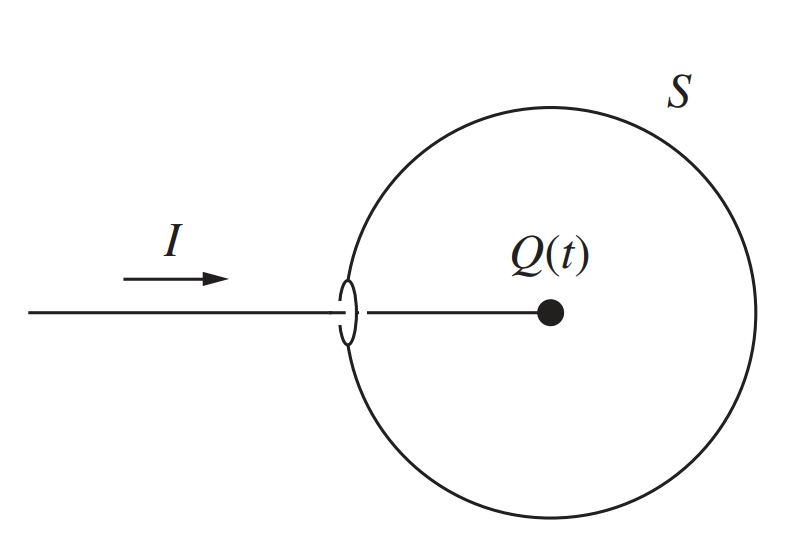
\includegraphics[width=5cm]{purcell_glassblo.png}
\end{center}
The circumference $C$ of this hole is the boundary of the surface $S$. Verify that the integral form of Maxwell’s equation,
$$\int_C \mathbf B \cdot \mathrm d \mathbf s = \int_S \left(\mu_0\epsilon_0 \frac{\partial \mathbf E}{\partial t} + \mu_0 \mathbf J\right)\cdot d\mathbf a.$$
is satisfied.

\end{prob}
\begin{sol}
    There is no enclosed current, so the right hand side is just the electric flux. Because the hole is small, we have
    $$\Phi_E \approx \frac{Q(t)}{\epsilon_0}.$$
    Furthermore, because it is also small, we have that the magnetic field is approximately $\mu_0 I/2\pi r$, which gives
    $$\int_C \mathbf \cdot\mathrm d \mathbf s = \frac{\mu_0 I}{2\pi r} (2\pi r) = \mu_0 I = \mu_0 \epsilon_0 \frac{dQ(t)/dt}{\epsilon_0} = \mu_0 \epsilon_0 \frac{d\Phi_E}{dt},$$
    as desired.
\end{sol}

\begin{prob}
    Consider the classical model of an atom. We have a negatively charged electron in a circular orbit about the positively charged proton. However, as we learned in class, because the electron has centripetal acceleration, it will be radiating away energy, given by the Larmor formula.
    \begin{anum}
        \item Assuming that the electron stays in an approximately circular orbit, determine how long it would take for the electron to spiral in from a radius $R$ to a radius $r$.
        \item Compare the velocity of the electron (assuming an orbital radius of 0.5 \AA) to the
speed of light – will relativistic corrections materially alter your conclusions?
\item What happens to the energy of the electron as it approaches the proton?
    \end{anum}
\end{prob}
\begin{alphasol}
    \item We have that the total energy of the system of the proton and the electron by the virial theorem is
    $$E = -\frac{e^2}{8\pi \epsilon_0 r}.$$
    So,
    $$\frac{dE}{dt} = \frac{e^2}{8\pi \epsilon_0 r^2}\frac{dr}{dt}.$$
    Then, using the Larmor formula, we can write down 
    $$\frac{dE}{dt} = -\frac{q^2a^2}{6\pi \epsilon_0 c^3} =-\frac{e^2}{6\pi\epsilon_0 c^3} \left(\frac{e^2}{4\pi \epsilon_0 r^2m_e}\right)^2 .$$
    Plugging this in, we get
    $$-\frac{e^2}{6\pi\epsilon_0 c^3} \left(\frac{e^2}{4\pi \epsilon_0 r^2m_e}\right)^2 = \frac{e^2}{8\pi\epsilon_0 r^2}\frac{dr}{dt} \implies -\frac{e^2}{6\pi\epsilon_0 c^3}\frac{e^2}{2\pi \epsilon_0m_e^2} = r^2\frac{dr}{dt} .$$
    Integrating from $R$ to $r$, we get
    $$\frac 13 (r^3 - R^3) = -\frac{e^2}{6\pi\epsilon_0 c^3}\frac{e^2}{2\pi \epsilon_0m_e^2}t,$$
    which gives $t$ upon division of the factor in front.
    \item At an orbital radius $r$, we can find the speed from
    $$\frac{v^2}{r} = \frac{e^2}{4\pi \epsilon_0 m_e r^2},$$
    which gives 
    $$v = \sqrt{\frac{e^2}{4\pi\epsilon_0 m_e r}} \approx 2 \times 10^6 \,\unit{m/s}.$$
    which is only $0.007$ of the speed of light, so we can neglect relativistic contributions.
    \item It approaches $-\infty$. Once it gets close enough other corrections should come into play. 
\end{alphasol}

\begin{prob}
    Here's a fascinating puzzle, first popularized by \href{https://www.youtube.com/watch?v=bHIhgxav9LY}{Veritasium}. Suppose you have a really long circuit as pictured below.
    \begin{center}
        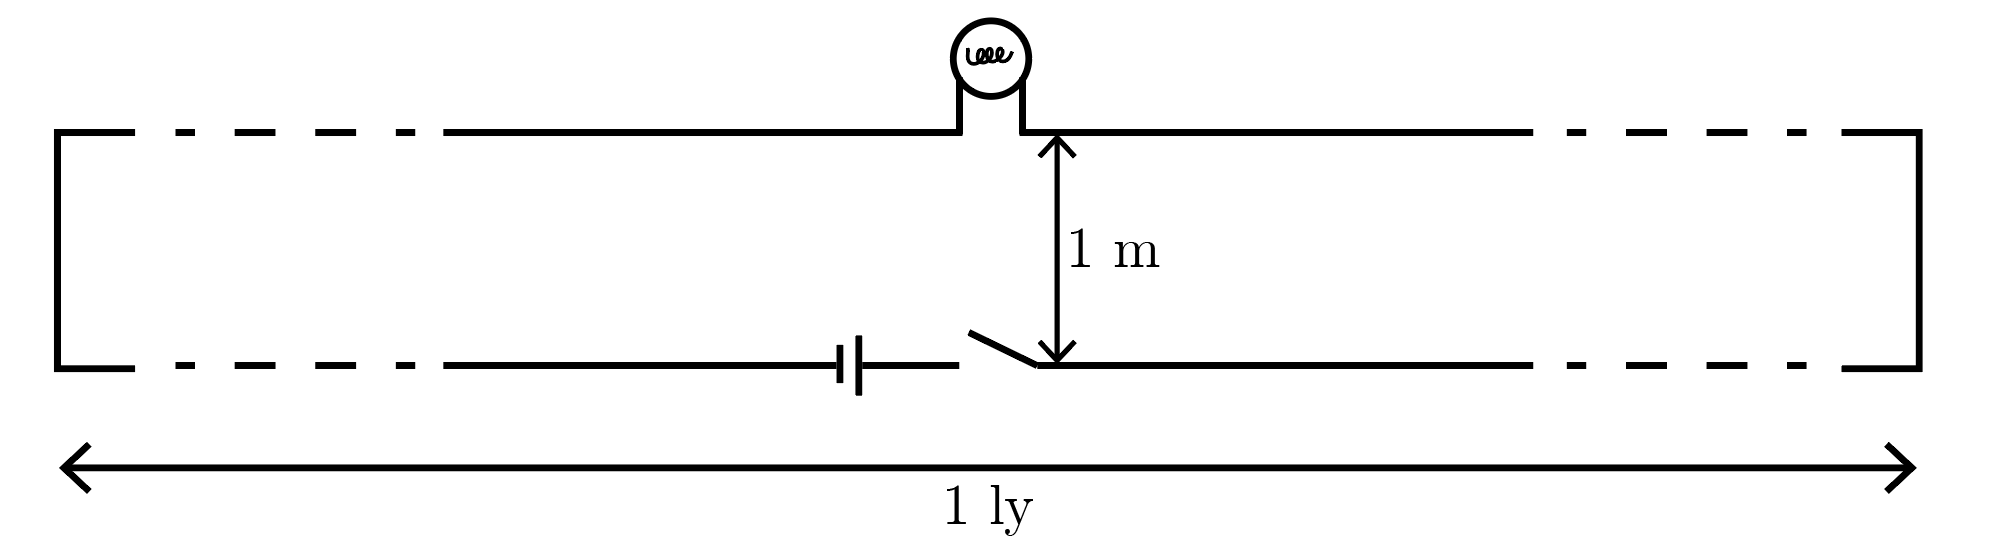
\includegraphics[height=4cm]{circuit_puzzle.png}
    \end{center}
    How long after the switch is closed does it take for the light bulb to light up?
    \begin{choices}
        \item 1 year
        \item 2 years
        \item $1/c$ seconds
        \item Other?
    \end{choices}
    Explain your answer.
\end{prob}
\begin{sol}
    The answer is (C)! Veritasium has two videos dedicated to this question: \url{https://www.youtube.com/watch?v=bHIhgxav9LY} and \url{https://www.youtube.com/watch?v=oI_X2cMHNe0}. The key here is to think about the poynting vector. The poynting vector represents the transmission of energy through electromagnetic fields, and fields travel at the speed of light. As you examined in problem \ref{pr:poynting_excs}, the poynting vector outside of the wires points away from them and thus toward the light bulb here. The electrons don't actually need to loop around for the light bulb to light up -- the electrons near the light bulb just need to be moved by some electric field, which gets there in $1/c$ seconds.
\end{sol}

\begin{prob}[Purcell]
    A half-infinite wire carries current $I$ from negative infinity to the
origin, where it builds up at a point charge with increasing $q$ (so
$dq/dt = I$). Consider the circle shown in Fig. 9.12, which has radius $b$ and subtends an angle $2\theta$ with respect to the charge. Calculate the integral $\int \mathbf B\cdot \mathrm d s$ around this circle. Do this in two ways.
\begin{center}
    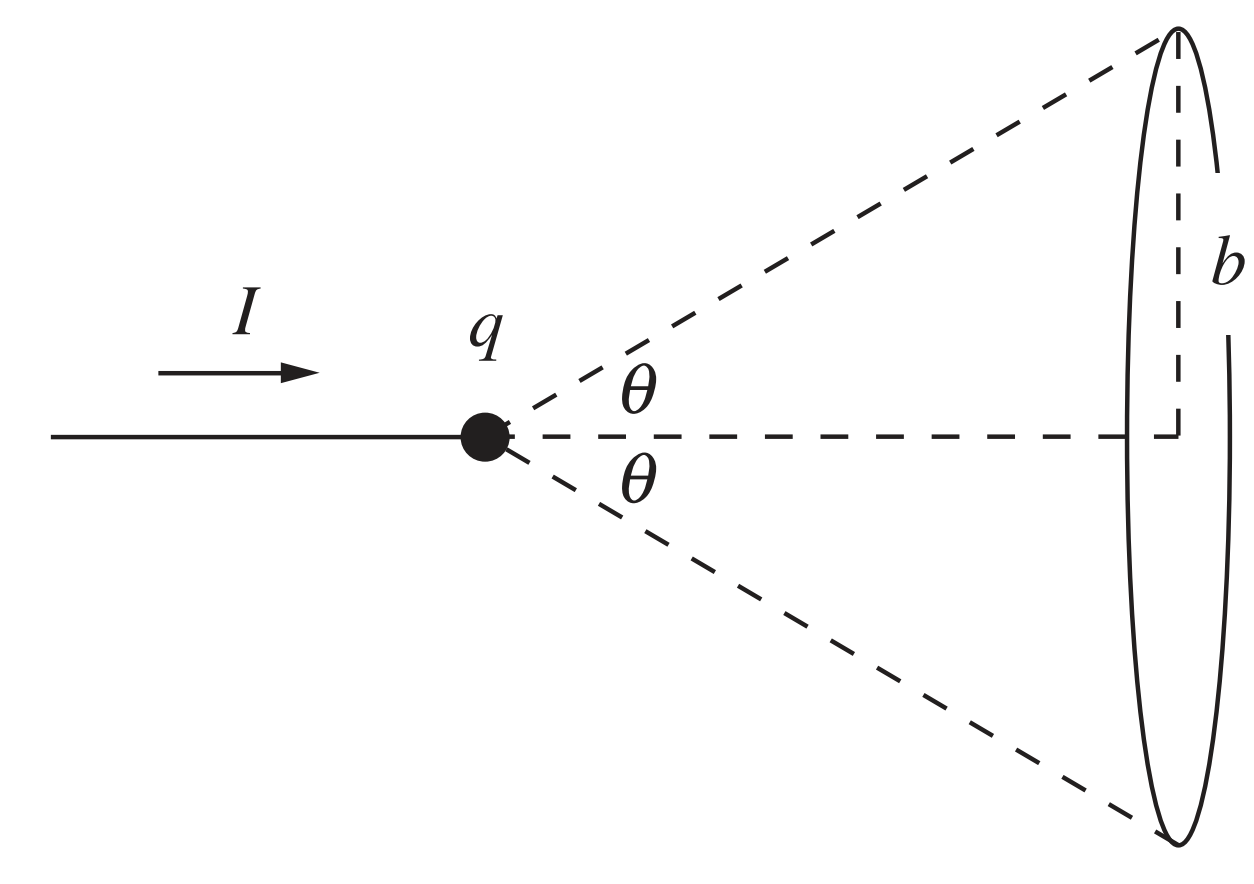
\includegraphics[width=6cm]{charge_buildiup.png}
\end{center}
\begin{anum}
    \item Use Ampere's Law with the given surface.
    \item Use Ampere's Law with a surface which intersects the wire.
\end{anum}
\end{prob}
\begin{alphasol}
    \item There is no current through this given surface, only the displacement current. Thus, we have
    $$\oint \mathbf B \cdot \mathrm d \mathbf s = \mu_0 \epsilon_0\frac{d\Phi_E}{dt}.$$
    Now, from week 1 electrostatics, we have
    $$\Phi_E = \frac{q(1-\cos \theta)}{2\epsilon_0}.$$
    So, plugging that in, we have
    $$B(2\pi b) = \mu_0 \frac{1-\cos \theta}{2} \frac{dq}{dt},$$
    so dividing, we get
    $$B = \frac{\mu_0 I(1-\cos \theta)}{4\pi b}.$$
    \item If we use a surface that intersects the wire, we have that the enclosed current is $I$. Now, for the flux, the total flux through a closed surface is $q/\epsilon_0$ by gauss's law, so the flux through the back part of the surface completed by the disk is
    $$\frac{q}{\epsilon_0} - \frac{q(1-\cos \theta )}{2} = \frac{q(1+\cos \theta)}{2}.$$
    So, Ampere's law now reads
    $$\oint \mathbf B \cdot \mathrm d \mathbf s = \mu_0 I - \mu_0 \frac{1+\cos \theta}{2} I = \frac{\mu_0 I(1-\cos \theta)}{4\pi b},$$
    which matches up with the previous part.
\end{alphasol}



\subsection{Tricky Non-linear Circuits}

\begin{prob}
    \href{https://www.ioc.ee/~kalda/ipho/es/NBPhO16-eng.pdf}{NBPhO 2016, problem 4}.
\end{prob}
\begin{sol}
    \officialsol{https://www.ioc.ee/~kalda/ipho/es/NBPhO16-sol.pdf}
\end{sol}


\begin{prob}[NBPhO]
    A Zener
diode is connected to a source of alternating current as shown in the figure. The current is sinusoidal $I = I_0 \cos \omega t$ with a constant amplitude.
The inductance $L$ of the inductor is such that
$L\omega I_0 \gg V_1,V_2$, where $V_1$ and $V_2$ are the breakdown voltages ($V_1 > V_2$). The current-voltage characteristic of the Zener diode is shown in the
figure. In the following assume that a very long
time has passed since the current source was first
turned on.
\begin{center}
    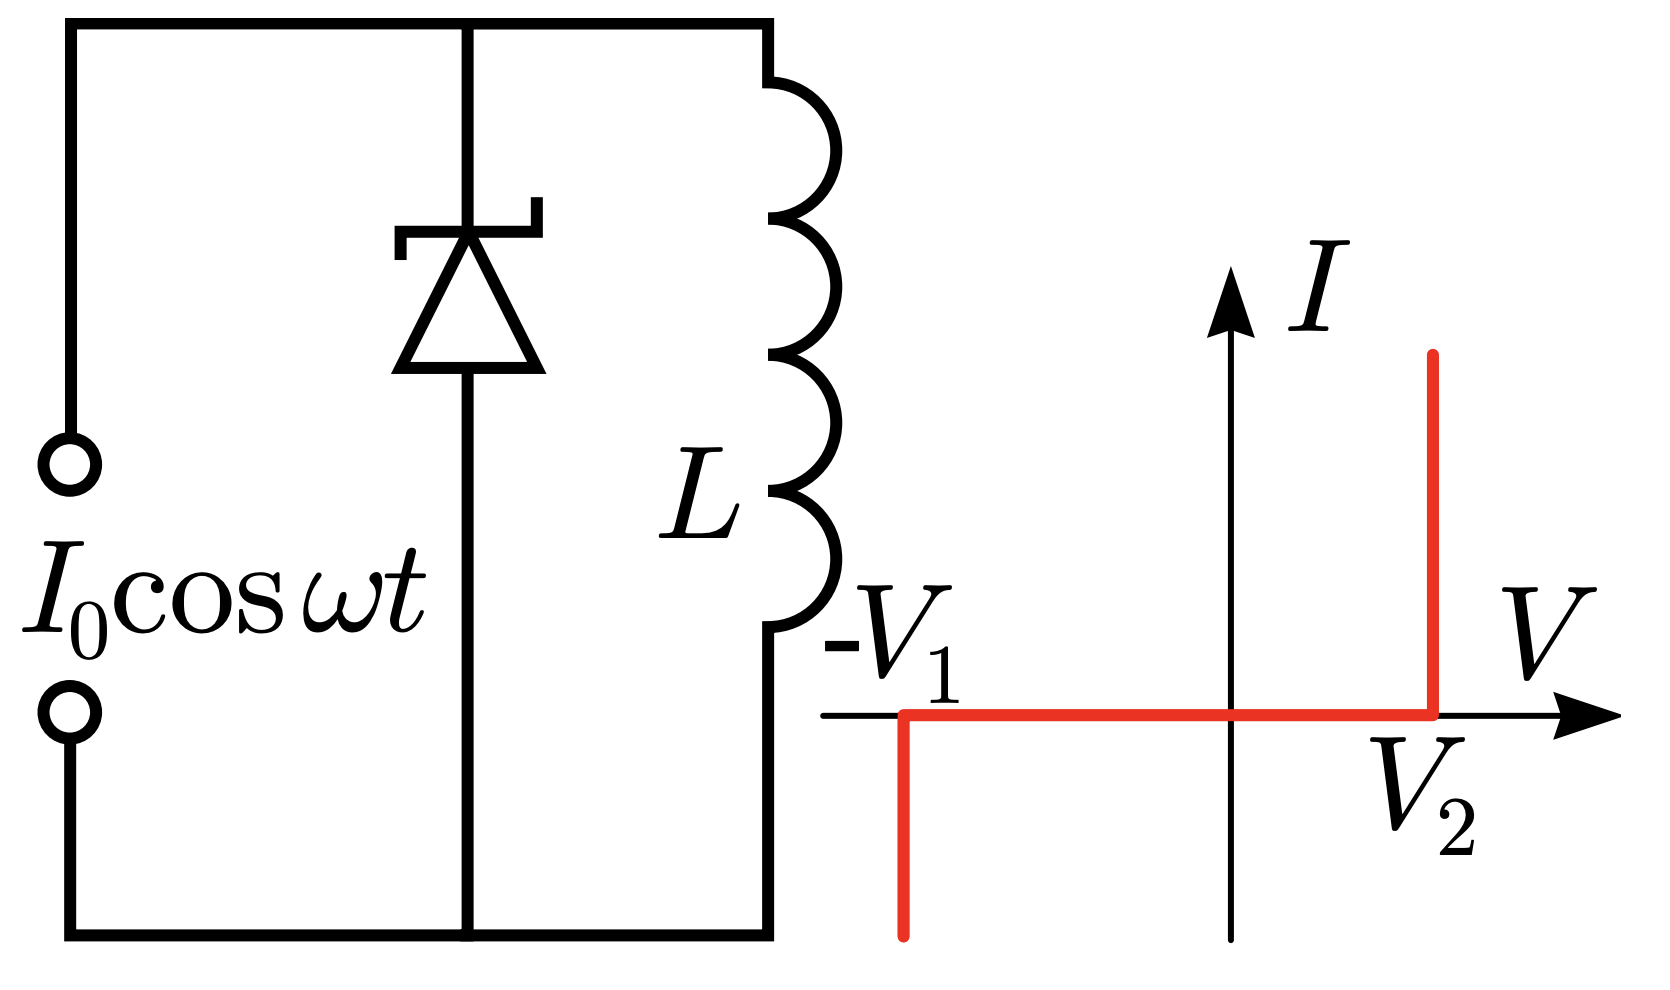
\includegraphics[width=6cm]{zener_nbpho.png}
\end{center}
\begin{anum}
    \item Find the time-averaged current $\langle I\rangle$ through the circuit.
    \item Find the peak-to-peak amplitude of
the current changes $\Delta I$ in the inductor.
\end{anum}
\end{prob}
\begin{sol}
    \officialsol{https://www.ioc.ee/~kalda/ipho/es/NBPhO17_sol.pdf}
\end{sol}

\begin{prob}
    Finish the last two parts of \href{https://www.ioc.ee/~kalda/ipho/es/es2010_eng.pdf}{EFPhO 2010, problem 9} that we started in class.
\end{prob}
\begin{sol}
    \officialsol{https://www.ioc.ee/~kalda/ipho/es/es2010_sol.pdf}
\end{sol}

\subsection{Challenge Problems}

% https://www.ioc.ee/~kalda/ipho/IPhO_1996_Theory.pdf
%potentially teach canonical angular momentum idea
\begin{prob}
    \href{https://ipho.olimpicos.net/pdf/IPhO_1996_Q2.pdf}{IPhO 1996/T2}, a question that references canonical angular momentum.
\end{prob}
\begin{sol}
    \officialsol{https://ipho.olimpicos.net/pdf/IPhO_1996_S2.pdf}
\end{sol}


\begin{prob}
    \href{https://www.aapt.org/Common2022/upload/2021-USAPhO_plus.pdf\#page=8}{2021 USAPhO+/T3}, a question that combines many of our previous weeks together.
\end{prob}
\begin{sol}
    \officialsol{https://aapt.org/Common2022/upload/2021-USAPhO_plus_Solutions_v2.pdf}
\end{sol}

%https://aapt.org/physicsteam/2021/upload/2021USAPhO_plus-solutions.pdf
%more canonical momentum

\begin{prob}
    \href{https://ipho.olimpicos.net/pdf/IPhO_2016_Q2.pdf}{IPhO 2016/T2}. This problem covers a tricky non-linear circuit element.
\end{prob}
\begin{sol}
    \officialsol{https://ipho.olimpicos.net/pdf/IPhO_2016_S2.pdf}
\end{sol}

\subsection{USAPhO Practice}

\begin{prob}[USAPhO 2016/A2]
    The problem is \href{https://www.aapt.org/physicsteam/2016/upload/E3-2-3.pdf\#page=4}{here}.
\end{prob}
\begin{sol}
\officialsol{https://aapt.org/physicsteam/2016/upload/E3-2-3.pdf\#page=4}
\end{sol}

\begin{prob}[USAPhO 2010/B2]
    These three parts can be answered independently.
    \begin{anum}
        \item One pair of ends of two long, parallel wires are connected by a resistor, $R = 0.25 \,\Omega$, and a
fuse that will break instantaneously if $5$ amperes of current pass through it. The other pair
of ends are unconnected. A conducting rod of mass m is free to slide along the wires under
the influence of gravity. The wires are separated by $30$ cm, and the rod starts out $10$ cm
from the resistor and fuse. The whole system is placed in a uniform, constant magnetic field
of $B = 1.2\, \unit{T}$ as shown in the figure. The resistance of the rod and the wires is negligible.
When the rod is released is falls under the influence of gravity, but never loses contact with
the long parallel wires.
\begin{center}
    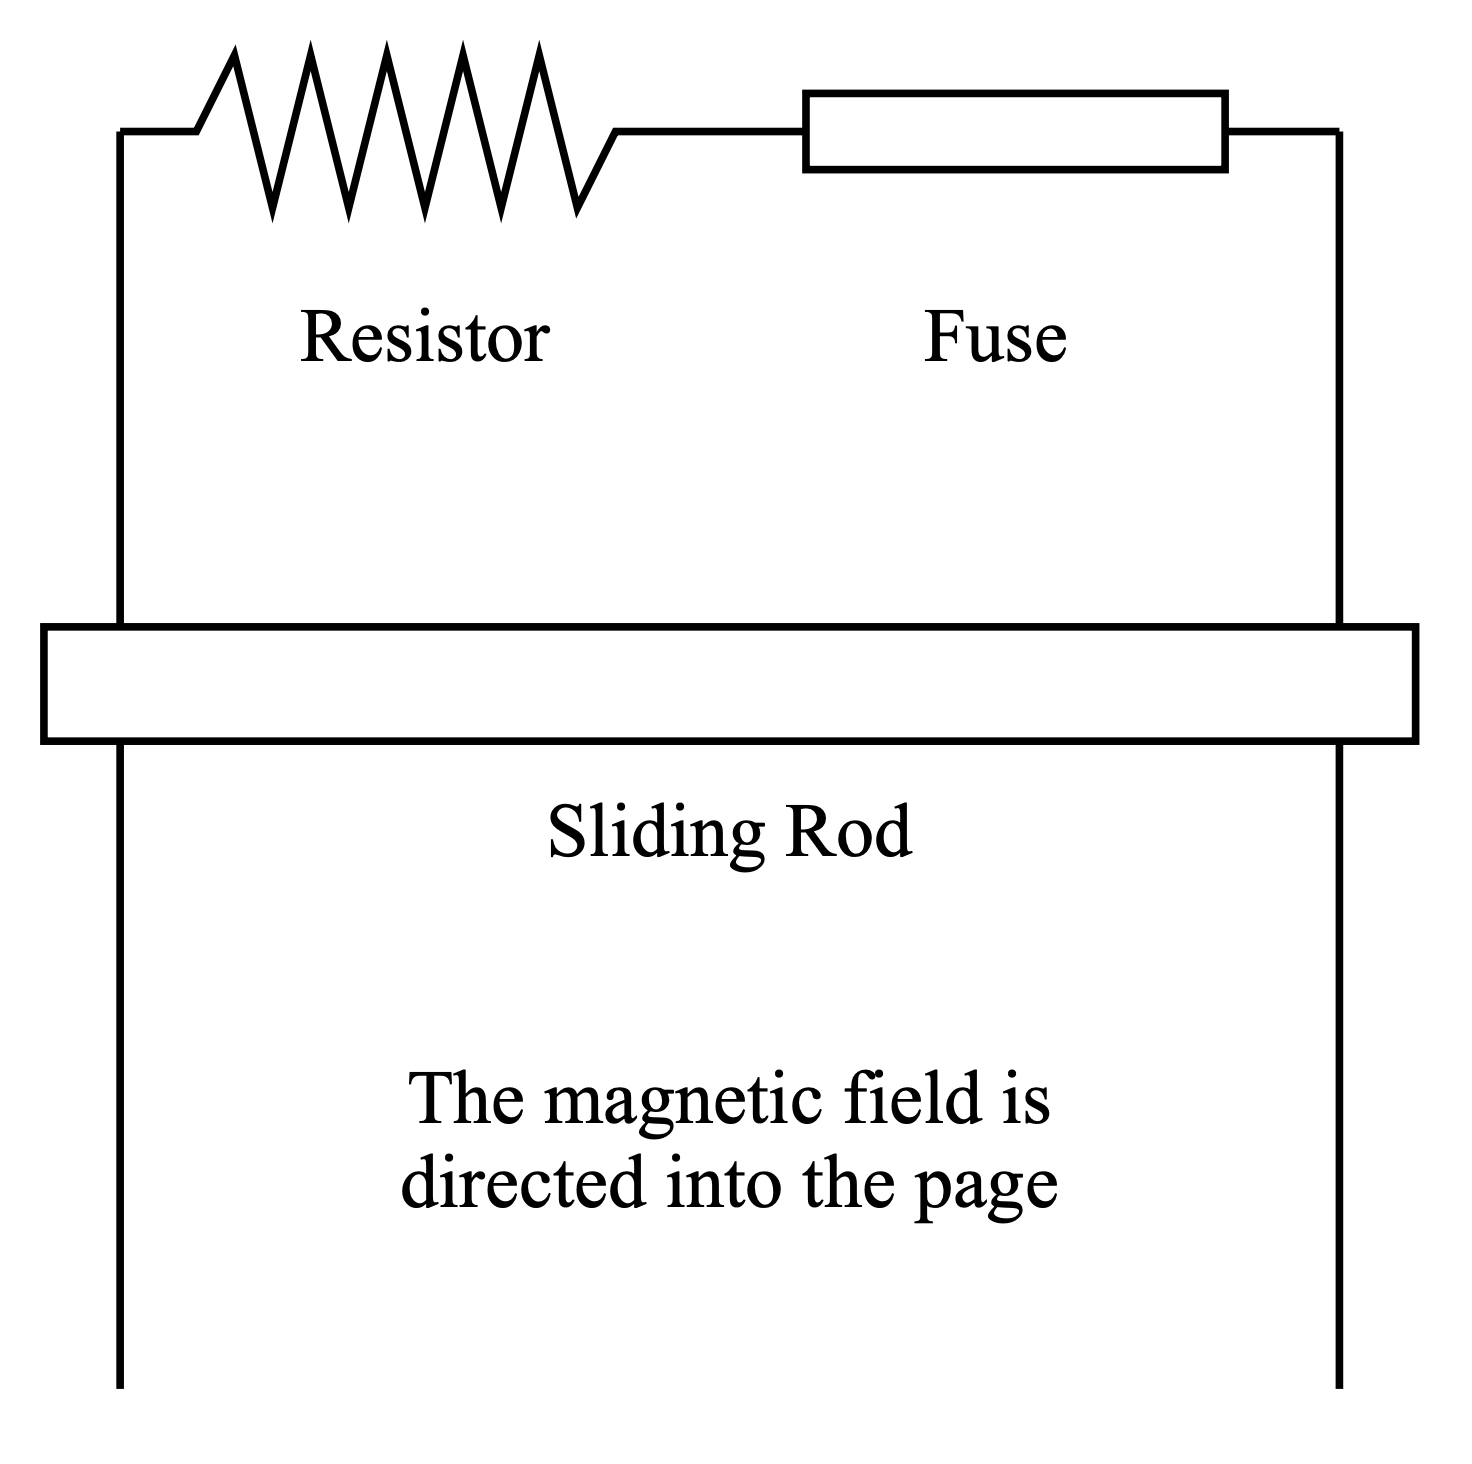
\includegraphics[width=6cm]{usapho_2010_b2.png}
\end{center}
\begin{enumerate}[label=\roman*.]
    \item What is the smallest mass needed to break the fuse?
    \item How fast is the mass moving when the fuse breaks?
\end{enumerate}
\item A fuse is composed of a cylindrical wire with length $L$ and radius $r \ll L$. The resistivity
(not resistance!) of the fuse is small, and given by $\rho_f$. Assume that a uniform current $I$ flows
through the fuse. Write your answers below in terms of $L$, $r$, $\rho_f$, $I$, and any fundamental constants.
\begin{enumerate}[label=\roman*.]
    \item What is the magnitude and direction of the electric field on the surface of the fuse wire?
    \item What is the magnitude and direction of the magnetic field on the surface of the fuse
wire?
\item The Poynting vector, $\vec{\mathbf S}$ is a measure of the rate of electromagnetic energy flow through
a unit surface area; the vector gives the direction of the energy flow. Since $\mathbf S = \frac 1 {\mu_0} \mathbf E \times \mathbf B$
where $\mu_0$ is the permeability of free space and and $\mathbf E$ and $\mathbf B$ are the electric and magnetic
field vectors, find the magnitude and direction of the Poynting vector associated with the current in the fuse wire.
\end{enumerate}
\item A fuse will break when it reaches its melting point. We know from modern physics that a
hot object will radiate energy (approximately) according to the black body law $P = \sigma AT^4$, where $T$ is the temperature in Kelvin, $A$ the surface area, and $\sigma$ is the Stefan-Boltzmann constant. If $T_f = 500\,\unit K$ is the melting point of the metal for the fuse wire, with resistivity $\rho_f = 120 \, \unit{n\Omega \cdot m}$, and $I_f = 5\, \unit A$ is the desired breaking current, what should be the radius of the wire $r$?
    \end{anum}
\end{prob}
\begin{sol}
    \officialsol{https://aapt.org/physicsteam/2019/upload/USAPhO-2010-Solutions.pdf\#page=11}
\end{sol}


\end{document}